\documentclass[10pt]{beamer}
\usetheme[
%%% options passed to the outer theme
%    hidetitle,           % hide the (short) title in the sidebar
%    hideauthor,          % hide the (short) author in the sidebar
%    hideinstitute,       % hide the (short) institute in the bottom of the sidebar
%    shownavsym,          % show the navigation symbols
%    width=2cm,           % width of the sidebar (default is 2 cm)
%    hideothersubsections,% hide all subsections but the subsections in the current section
%    hideallsubsections,  % hide all subsections
%    left                % right of left position of sidebar (default is right)
  ]{Aalborg}
  
% If you want to change the colors of the various elements in the theme, edit and uncomment the following lines
% Change the bar and sidebar colors:
%\setbeamercolor{Aalborg}{fg=red!20,bg=red}
%\setbeamercolor{sidebar}{bg=red!20}
% Change the color of the structural elements:
%\setbeamercolor{structure}{fg=red}
% Change the frame title text color:
%\setbeamercolor{frametitle}{fg=blue}
% Change the normal text color background:
%\setbeamercolor{normal text}{bg=gray!10}
% ... and you can of course change a lot more - see the beamer user manual.

\usepackage[utf8]{inputenc}
\usepackage[english]{babel}
\usepackage[T1]{fontenc}
% Or whatever. Note that the encoding and the font should match. If T1
% does not look nice, try deleting the line with the fontenc.
\usepackage{helvet}


% colored hyperlinks
\newcommand{\chref}[2]{%
  \href{#1}{{\usebeamercolor[bg]{Aalborg}#2}}%
}

\title[Semantic Web Mining]% optional, use only with long paper titles
{Semantic Web Mining}

\subtitle{Semantic Web Course}  % could also be a conference name

\date{\today}

\author[Ali Mohebbi, Mehdi Keshani] 
 % optional, use only with lots of authors
{
  Ali Mohebbi\\
  \href{mailto:a.mohebbi@ce.sharif.edu}{{\tt a.mohebbi@ce.sharif.edu}}\\
   Mehdi Keshani\\
  \href{mailto:keshani@ce.sharif.edu}{{\tt keshani@ce.sharif.edu}}
}

% - Give the names in the same order as they appear in the paper.
% - Use the \inst{?} command only if the authors have different
%   affiliation. See the beamer manual for an example

\institute[
%  {\includegraphics[scale=0.2]{aau_segl}}\\ %insert a company, department or university logo
  Dept.\ of Computer Engineering\\
  Sharif University\\
  Iran
] % optional - is placed in the bottom of the sidebar on every slide
{% is placed on the bottom of the title page
  Dept.\ of Computer Engineering\\
  Sharif University\\
  Iran
  
  %there must be an empty line above this line - otherwise some unwanted space is added between the university and the country (I do not know why;( )
}

% specify the logo in the top right/left of the slide
\pgfdeclareimage[height=1cm]{mainlogo}{AAUgraphics/aau_logo_new} % placed in the upper left/right corner
\logo{\pgfuseimage{mainlogo}}

% specify a logo on the titlepage (you can specify additional logos an include them in 
% institute command below
\pgfdeclareimage[height=1.5cm]{titlepagelogo}{AAUgraphics/aau_logo_new} % placed on the title page
%\pgfdeclareimage[height=1.5cm]{titlepagelogo2}{AAUgraphics/aau_logo_new} % placed on the title page
\titlegraphic{% is placed on the bottom of the title page
  \pgfuseimage{titlepagelogo}
%  \hspace{1cm}\pgfuseimage{titlepagelogo2}
}
\usepackage{ragged2e}
\usepackage{etoolbox}
\usepackage{lipsum}
\apptocmd{\frame}{}{\justifying}{}
\begin{document}
% the titlepage
{\aauwavesbg
\begin{frame}[plain,noframenumbering] % the plain option removes the sidebar and header from the title page
  \titlepage
\end{frame}}
%%%%%%%%%%%%%%%%

% TOC
\begin{frame}{Agenda}{}
\tableofcontents
\end{frame}
%%%%%%%%%%%%%%%%


\section{Data Mining}
\subsection{Classification}
\begin{frame}{Data Mining}{Classification}

\end{frame}
\subsection{Clustring}
\begin{frame}{Data Mining}{Clustering}

\end{frame}
\subsection{Association Rule Mining}
\begin{frame}{Data Mining}{Association Rule Mining}

\end{frame}
\section{Semantic Web Mining}

\begin{frame}{Semantic Web Mining}
\begin{itemize}
	\item Semantic web in data mining
	\begin{itemize}
		\item Concerned with deriving higher-level insights from data
		\item Are knowledge intensive and can often benefit from using additional knowledge from various sources
		\item Document classification, Document clustering
	\end{itemize}
	\item Data mining in semantic web
	\begin{itemize}
		\item Building ontologies is a time consuming task
		\item Data mining techniques could be fruitfully exploited for learning models from existing Web data
		\item Models can be used for building and enriching ontologies from
	\end{itemize}
\end{itemize}
\end{frame}

\subsection{ِData mining in Semantic Web}
\begin{frame}{Semantic Web Mining}{Data mining in Semantic Web}
	 \begin{itemize}
		\item In presence of noisy/inconsistent knowledge bases, that could be highly probable in  the Web, deductive reasoning is no more applicable 
		\item inductive reasoning is grounded on the generalization of specific examples (assertions in the SW context) allowing the formulation of conclusions even when inconsistent/noisy knowledge bases are considered
		\item The main focus is on   building the terminology of an ontology while less attention has been dedicated to the enrichment/construction of the assertional part
		\item enrichment/construction of the assertional part, namely the ontology population problem results in an even more time consuming task
	 \end{itemize}
\end{frame}

\subsection{Classification}
\begin{frame}{Semantic Web Mining}{Classification}
	\begin{itemize}
		\item Ontology population task: the problem has been focused by casting it to a classification problem
	 	\item Requires some assumption
	 		\begin{enumerate}
				\item Open world assumption
				\item Non-disjointness of the classes
				\item the availability of new similarity measures to exploit the expressiveness of DLs 
	 		\end{enumerate}
 		\item Nearest Neighbor (NN) and Support Vector Machine have been used in studies.
	\end{itemize}
\end{frame}
\subsection{Clustering}
\begin{frame}{Semantic Web Mining}{Clustering}
	\begin{itemize}
	\item Ontology learning task: focuses on learning ontologies (mainly terminologies) from text documents by the use of clustering methods
		\begin{enumerate}
			\item Concepts are extracted from documents by the use of Natural Language Processing techniques   
			\item Concept are clustered to obtain an initial terminology 
			\item Enriched with new relationships  by means of association rules
		\end{enumerate}
	\item There are some drawbacks 
		\begin{enumerate}
			\item Semantic relations among the terms are not fully clear 
			\item Expressiveness of the adopted language is less than OWL
		\end{enumerate}
	\end{itemize}
\end{frame}

\subsection{Association Rule Mining}
\begin{frame}{Semantic Web Mining}{Association Rule Mining}
\end{frame}

\section{Association Rule Mining}
\subsection{Challenges}
\begin{frame}{Association Rule Mining}{Challenges}


\end{frame}


\subsection{Related Works}


\begin{frame}{Association Rule Mining}{Related Works}
\begin{itemize}
\item
\end{itemize}

\begin{figure}[H]
	\centering
	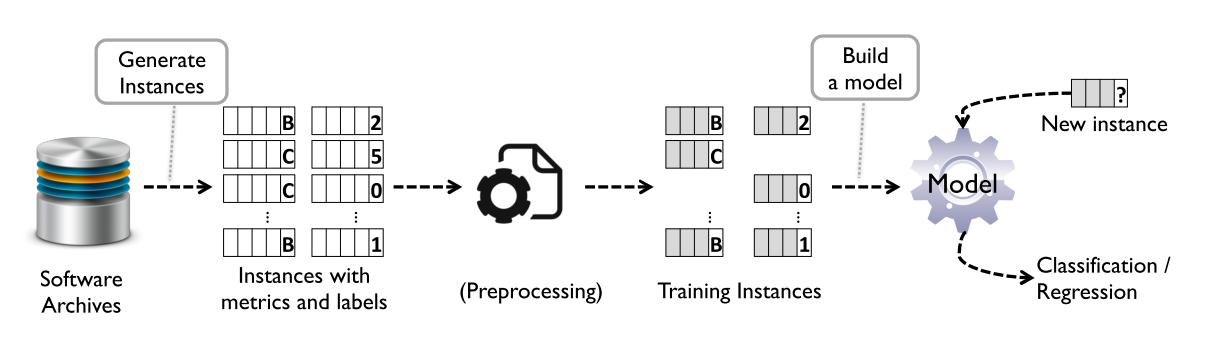
\includegraphics[width=1.0\textwidth]{images/prediction-process.PNG}
	\caption{process \cite{nam2014survey}}
	\label{fig:prediction-process}
\end{figure}

\end{frame}

\section{References}
 \begin{frame}[allowframebreaks] {References}
 \bibliographystyle{plain}
\bibliography{References}
\end{frame}
%%%%%%%%%%%%%%%%

{\aauwavesbg%
\begin{frame}[plain,noframenumbering]%
  \finalpage{Thank you.}
\end{frame}}
%%%%%%%%%%%%%%%%

\end{document}
